% ************ Chapter 2 ************
%\renewcommand{\chaptername}{Chapter}
\chapter{Estado da Arte}
\label{cap:2}
\emph{
O tema descentralização da web não é novo, existindo até ao momento alguns projetos relevantes nesta área.
Este capitulo consiste numa apresentação mais detalhada sobre a alternativas que demonstram mais potencial.
É expectável que os detalhes estudados e apresentados permitam tirar mais conclusões no capitulo correspondente à análise de valor. }

Assistimos hoje em dia a problemas sérios e crescentes relativos a manipulação de informação, consequentes de um paradigma de web que foi explorado ao limite, por forma a criar modelos de negócio obscuros e com pouca transparência na recolha e utilização dos dados de utilizadores.

O modelo actual é um monstro gigante, onde a informação se encontra replicada infinitamente, e a camada de persistência de dados nas diferentes arquiteturas é provavelmente aquela que mais destaque tem para todas as estruturas organizacionais, na medida em que persiste o ativo principal das empresas, os dados relativos a toda a atividade todos seus clientes. \cite{top_three_issues_centralized_web}. Isto torna-se um problema, quando não existe respeito pelos utilizadores e a manipulação dos dados passa a ser o "core business". Esta manipulação pode ser positiva, no sentido de criar valor para a empresa e para o cliente, ou pode ser negativa se estivermos perante casos de uso de que invadam a privacidade ou que cedam os dados a terceiros não devidamente autorizados \cite{facebook_data_hell_medium}.

Um modelo de descentralização da web, vem sendo discutido desde tempos atrás, com várias abordagens possíveis, mas sempre com a garantia de que a informação será sempre propriedade do utilizador. \cite{why_web_decentralization_future}
|A emersão de um novo modelo para a web, está dependente da migração do "antigo" para o novo, sendo que esta migração teria de ser massiva para o modelo descentralizado ter sucesso, na medida em que estaria pendente da aceitação de plataformas digitais com infraestruturas de dimensão considerável e de toda a comunidade de engenharia informática. Esta adoção massiva por sua vez requer um conjunto de ferramentas capazes de sustentar o seu funcionamento de forma eficaz e suficientemente escalável \cite{shift_power_to_users}.

\section{Modelos Descentralizados}
Nesta secção são apresentadas diferentes alternativas que podem servir de base para um novo paradigma de web descentralizada. Para tal devem ser soluções robustas e que ofereçam ferramentas auxiliares para o desenvolvimento e posterior integração de novas aplicações.

\subsection{Solid}
A arquitetura implícita para o desenvolvimento de aplicações baseadas em Solid permite que os utilizadores escolham um POD (\emph{Personal online datastore} \label{sym:POD})  à sua escolha (próprio ou recorrendo a um servidor de POD \label{sym:POD}) para conceder às aplicações autorização para armazenar ou ler informação a partir do mesmo. Por si só, este facto permite que os utilizadores escapem dos tradicionais "silos de dados". Além disto, esses PODs \label{sym:POD} podem oferecer diferentes granularidades de privacidade, confiabilidade, disponibilidade, proteção legal e reutilização de dados \cite{solid_official}. Desta forma este componente do Solid, confere a camada de persistência de informação dos utilizadores, podendo inclusive ser viste como o novo \emph{backend} das aplicações, que poderão aceder à informação através da interface Rest \cite{rest_foundations} disponibilizada por cada POD, baseada em Linked Data Platform (LDP \label{sym:LDP}), uma recomendação da comunidade W3C, assim como um mecanismo baseado em queries SPARQL.\cite{solid_spec}

\subsubsection{Autenticação}
A identidade dos utilizadores no Solid baseia-se em URIs WebID, estes funcionam como nomes universais que permitem identificar determinado utilizador de forma descentralizada. Segue-se um exemplo de um possível WebID:

\emph{https://john.domain.com/profile/card\#me}

Neste sentido, o Solid, tratando-se de uma plataforma descentralizada, tem requisitos diferentes da maioria das aplicações existentes. Mais propriamente, precisa de estar assente em mecanismos de autenticação \emph{cross-domain} suficientemente descentralizados e isolados de qualquer serviço ou entidade.\cite{solid_spec}

Até ao momento, o mecanismo de autenticação a ser utilizado em determinada instância de um POD, pode ser um de dois: WebID-TLS ou WebID-OIDC. Esta capacidade de abstração ao mecanismo de autenticação, permite que possam continuamente ser estudados e adotados novos mecanismos que se entenda relevantes.\cite{solid_spec}

\paragraph{\emph{WebID-TLS}}
foi o primeiro mecanismo de autenticação a ser implementado no Solid. Como forma de autenticar os WebIDs, em vez das tradicionais passwords recorre a certificados criptográficos (guardados e geridos no navegador web do utilizador) para comprovar a identidade do utilizador.\cite{solid_webid-tls:}

Este mecanismo, apesar de poder ainda ser utilizado, deixou de ser a configuração por omissão para instanciações de novos PODs. Isto, porque muitos navegadores web removeram suporte ao elemento \emph{KEYGEN}, que servia como base para este protocolo gerar certificados através do navegador web.\cite{solid_webid-tls:}

\paragraph{\emph{WebID-OIDC}}
é também um mecanismo de autenticação baseado WebID, tendo a particularidade de ser baseado no protocolo OpenID connect (OIDC). Este mecanismo adiciona ao fluxo normal de OIDC um passo extra que permite obter um URI WebID através de um token OIDC.\cite{solid_webid_oidc}

Seguem-se alguns dos conceitos mais relevantes neste protocolo:
\begin{itemize}
    \item \emph{User} - Utilizador humano (pode ser também uma aplicação ou serviço se estes tiverem o seu próprio webID). Também chamado \emph{Resource Owner}
    \item \emph{User-Agent} - Nome formal para navegador Web.
    \item \emph{Identity Provider (OP)} - Um servidor de identidade baseado no protocolo OpenID Connect. Pode ser utilizado o próprio POD uma instância externa.
    \item \emph{Resource Server} - Um servidor responsável por alojar recursos que o utilizador precisa eventualmente de aceder, tais como HTML, imagens, \emph{Linked Data} / \emph{RDF sources}, entre outros tipos de recursos.
    \item \emph{Relying Party (RP)} - É um POD ou uma aplicação cliente que assenta a sua lógica num token providenciado por um servidor de identidade.
    \item \emph{POD} - Unidade online de armazenamento pessoal. Este componente do sistema desempenha vários papeis na arquitetura atual: armazena informação do utilizador (actua como \emph{Resource Server}), instancia um servidor de identidade webID-OIDC e pode também actuar como \emph{Relying Party} quando um utilizador requisita recursos a partir de um token.
\end{itemize}

\begin{figure}[h]
    \begin{center}
    % Requires \usepackage{graphicx}
    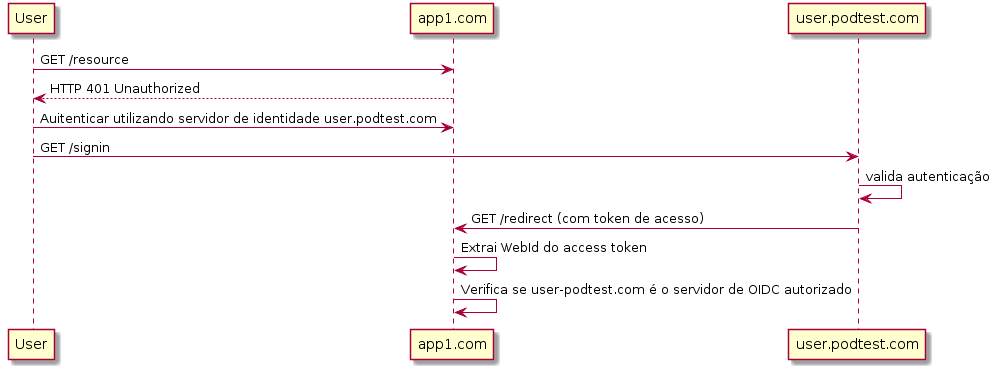
\includegraphics[width=1 \textwidth]{figures/WedId-OIDC.png}
    \caption{Diagrama de Sequência WebId-OIDC}
    \end{center}
\end{figure}

\pagebreak

Conforme é possível perceber pela figura acima, assemelha-se bastante ao protocolo OpenId Connect, adicionando dois passos extra:\cite{solid_webid_oidc}
\begin{itemize}
    \item Obter o WebId através do token de acesso
    \item Verificar se o servidor indicado para autenticação é de facto o servidor de identidade autorizado para o WebId em questão
\end{itemize}

\subsubsection{Autorização}
A autorização no Solid é garantida por uma peça com o nome \emph{Web Access Control (WAC)}, este componente consiste num sistema de controlo de acesso entre domínios de origem cruzada. Os seus conceitos principais baseiam-se em modelos de controlo de acesso a diferentes sistemas de ficheiros e as suas principais responsabilidades consistem em garantir acesso a agentes (utilizadores, grupos, entre outros) para conseguirem realizar ações (ler, escrever, editar, eliminar, entre outras).\cite{solid_web_access_control}
Seguem-se algumas das suas principais características:
\begin{itemize}
    \item Os recursos são identificados por URLs, e podem referir-se a qualquer recursos disponível na web;
    \item As políticas de controlo de acesso seguem uma estrutura declarativa;
    \item Utilizadores e grupos são também identificados URLs (WebIds);
    \item Agnóstico em termos de domínio, ou seja, as politicas de acesso a um determinado ficheiro podem conter utilizadores e grupos alojados em qualquer servidor de identidade existente.
\end{itemize}

\subsubsection{Armazenamento}
O Solid lida com dois tipos de informação:
\begin{itemize}
    \item Recursos \emph{Linked Data}
    \item Todo o restante tipo de informação
\end{itemize}
Desta forma, é possível construir aplicações baseadas em Solid com ou sem recursos sob a forma de \emph{Linked Data}.\cite{solid_spec}

Os recursos são agrupados em contentores baseados em directórios (cumprindo a especificação \emph{LDP Basic Container Spec}.\cite{solid_spec}

\begin{figure}[h]
    \begin{center}
    % Requires \usepackage{graphicx}
    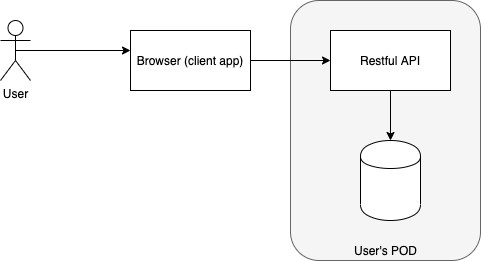
\includegraphics[width=1\textwidth]{figures/estado_arte-Solid.png}
    \caption{Representação SOLID}
    \end{center}
\end{figure}

\pagebreak

\subsection{Blockstack}
Blockstack é um projeto open-source que pretende construir uma rede de computação descentralizada assente na camada de transporte da Internet e protocolos de comunicação subjacentes. Para atingir este estatuto, está assente nas seguintes camadas:
\begin{description}
	\item Stacks Blockchain - Permite aos utilizadores controlar e register ativos digitais, como usernames e passwords ou executar contratos inteligentes.\cite{blockstack_white_paper};
	\item Gaia - Armazenamento descentralizado;
	\item Blockstack Authentication - Protocolo que permite autenticação descentralizada.\cite{blockstack_white_paper};
	\item Libraries and SDKs - Ferramentas para facilitar o desenvolvimento de aplicações baseadas em Blockstack \cite{blockstack_white_paper}.
\end{description}

Um dos conceitos chave da arquitetura desta plataforma é o sistema de ficheiros descentralizado chamado Gaia Hub, que permite aos utilizadores escolher e providenciar o seu repositório de informação.

Blockstack tem um sistema de armazenamento descentralizado baseado em Gaia Hubs, repositórios de informação privados que podem também ser partilhados entre a comunidade ou podem apenas ser propriedade de cada utilizador. 

Estes repositórios disponibilizam uma interface de aplicação RESTful, permitindo que as aplicações adicionem informação através de pedidos POST, sendo que cada pedido deve ser acompanhado por um token autenticação assinado e validado pelo repositório. Cada aplicação tem uma chave privada que confere acesso a uma partição especifica do repositório impedindo que, ao contrário do Solid, possa haver partilha de informação entre as diferentes aplicações.\cite{blockstack_white_paper}

Em termos de autenticação, o Blockstack consegue providenciar autenticação descentralizada através do mecanismo de autenticação por chave pública criptográfica. A partir do login, a aplicação recebe três peças essenciais de informação: o nome de utilizador, uma chave privada específica de aplicação e a localização do repositório para armazenar informação.\cite{blockstack_white_paper}

\begin{figure}[h]
    \begin{center}
    % Requires \usepackage{graphicx}
    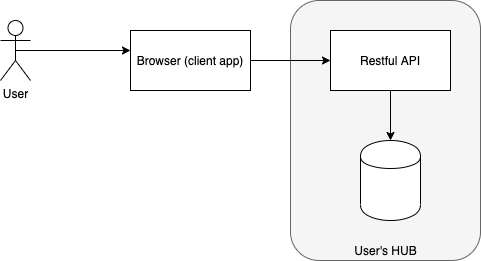
\includegraphics[width=1\textwidth]{figures/estado_arte-Blockstack.png}
    \caption{Representação Blockstack}
    \end{center}
\end{figure}

\subsection{Diaspora}
Diaspora é um projeto com uma visão um pouco mais reduzida que as restantes alternativas, na medida em que foca-se apenas em apresentar um protótipo daquilo que poderia ser uma rede social descentralizada. Este projeto assenta em servidores de informação independentes, que o utilizador pode escolher ou até mesmo configurar o seu. \cite{diaspora_wiki}

O conceito principal desta rede é o POD \label{sym:POD} (assim como no Solid), a sua arquitetura é relativamente intuitiva, tendo as aplicações a interagir com as instâncias servidoras distribuídas pelo mundo. Estes servidores são mantidos em sincronização utilizando a tecnologia WebSub. \cite{diaspora_wiki}

Relativamente a autenticação, não é adotado nenhum mecanismo fora do comum, sendo apenas o método comum username/password.

\begin{figure}[h]
    \begin{center}
    % Requires \usepackage{graphicx}
    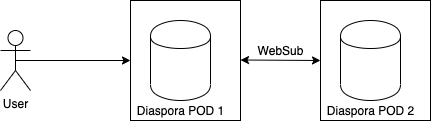
\includegraphics[width=1\textwidth]{figures/estado_arte-Diaspora.png}
    \caption{Representação Diaspora}
    \end{center}
\end{figure}

\subsection{Elastos}
Elastos incide no desenvolvimento de um novo paradigma de web potenciado por tecnologia \emph{blockchain}\cite{a_bit_about_blockchain}. O foco principal incide não só na proteção dos dados, mas também na defesa dos direitos de autor. A plataforma é constituída por quatro componentes:\cite{elastos_white_paper}
\begin{itemize}
	\item Elastos Blockchain
	\item Elastos Runtime
	\item Elastos Carrier
	\item Elastos SDK
\end{itemize}

O conceito baseia-se num sistema operativo relativamente leve que armazena a informação e previne que as aplicações e serviços tenham ligação à Internet. Toda a informação tem identificadores providenciados por Blockchain (pode ser Bitcoin ou uma rede de Blockchain alternativa \footnote{Qualquer outra rede Blockchain, não necessariamente a que serve de base à conhecida criptomoeda Bitcoin}), sendo estes IDs verificados antes de os ativos digitais serem transmitidos entre as diferentes máquinas virtuais, utilizando comunicação P2P ("\emph{Peer to Peer}" \label{sym:P2P})\cite{what_are_P2P_networks} providenciada pela camada Elastos Carrier.\cite{elastos_developer}

Elastos dispõe de um componente de armazenamento descentralizado, i.e. Elastos Hive. Recorre a um sistema de arquivos interplanetário (IPFS \label{sym:IPFS}) \cite{ipfs} como base. Oferece uma interface de aplicação para aceder à informação que será dispersa pelas diferentes regiões do planeta, garantindo assim fiabilidade às aplicações.\cite{elastos_white_paper}

Relativamente à autenticação, esta plataforma introduz um ID descentralizado (DID), construído na rede Blockchain e providencia IDs confiáveis para tudo e para todos. 

O ID pode ser utilizado para efeitos de rastreamento, autenticação e estabelecimento de ligações seguras. De forma simplificada, a camada Elastos Carrier é a combinação entre DID e a comunicação P2P, assegurando assim que a informação é transmitida em segurança após a autenticação e a autorização serem devidamente validadas.\cite{elastos_white_paper}

\begin{figure}[h]
    \begin{center}
    % Requires \usepackage{graphicx}
    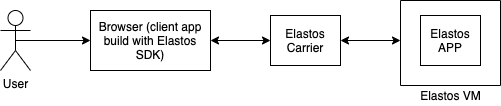
\includegraphics[width=1\textwidth]{figures/estado_arte-Elastos.png}
    \caption{Representação Elastos}
    \end{center}
\end{figure}

\subsection{Comparação Alternativas}

As diferentes serão de seguida comparada, sob a forma de tabela, em função de 3 características principais: Autenticação, Autorização, Armazenamento.



\begin{center}
\small
\begin{longtable}{c|p{4cm}|p{4cm}|p{4cm}}
\toprule 
    \multicolumn{1}{c}{-} &
    \multicolumn{1}{c}{Autenticação} &
    \multicolumn{1}{c}{Autorização} &
    \multicolumn{1}{c}{Armazenamento}
    \\ \midrule\addlinespace[2pt] \endhead

\bottomrule\endfoot

Solid & Os utilizadores são identificados através de um WebId. Autenticação baseada em camada abstrata que permite utilizar o protocolo WebId-TLS ou WebId-OIDC \cite{solid_spec}. &  Garantida por um sistema WAC (\emph{Web Access Control} \label{sym:WAC}). Este sistema por sua vez é composto por documentos que contêm regras sobre a forma declarativas, denominadas ACLs \label{sym:ACL}, que indicam o tipo de acesso que cada WebId tem a determinado recurso \cite{solid_web_access_control}. & PODs disponibilizam uma camada de persistência baseada em \label{sym:LDP}. Esta camada é acessível através de uma interface Rest. \cite{solid_spec} \\
Blockstack & Autenticação descentralizada através do mecanismo de autenticação por chave pública criptográfica \cite{blockstack_white_paper}. & Chave privada específica de aplicação confere o acesso a determinada partição do repositório e, consequentemente, aos seus recursos \cite{blockstack_white_paper}. & Sistema de ficheiros descentralizado chamado Gaia Hub, que permite aos utilizadores escolher e providenciar o seu repositório de informação \cite{blockstack_white_paper}. \\
Diaspora & Não é adotado nenhum mecanismo fora do comum, sendo apenas o método comum username/password \cite{diaspora_wiki}. & Autorização de acesso baseada no conceito \emph{Aspect}, este funciona como um agrupador de utilizadores que tem acesso a um determinado recurso \cite{diaspora_wiki}. & Os diferentes PODs \label{sym:POD} existentes pelo mundo conferem o funcionamento da rede social e mantem-se sincronizados utilizando a tecnologia WebSub \cite{diaspora_wiki}. \\
Elastos & Introduz um ID descentralizado (DID), construído na rede Blockchain e providencia IDs confiáveis para tudo e para todos \cite{elastos_white_paper}. & A camada \emph{Elastos Runtime contém um sistema de gestão de permissões que confere ou o acesso de determinado utilizador a um recurso} \cite{elastos_white_paper} & Recorre a um sistema de arquivos interplanetário (IPFS \label{sym:IPFS}) como base. \cite{elastos_developer} \\

\end{longtable}

\end{center}

\section{Métodos, Técnicas e Tecnologias}
No decorrer do desenvolvimento do projeto, foram constantemente estudados métodos, técnicas e tecnologias, de forma a responder a diferentes necessidades surgidas nas diferentes fases. Esta secção tem como propósito agrupar e explicar esses conceitos.

\subsection{Análise}
Nesta subsecção conceitos relativos à análise de valor do projeto (Capítulo 3), Sendo, desta forma, apresentados os seguintes: \emph{New Concept Development}, AHP (\emph{Analytic Hierarchy  Process} \label{sym:AHP}, modelo \emph{FAST} e o modelo de negócio Canvas

\subsubsection{New Concept Development}
O processo de inovação é divido em três componentes: \emph{Fuzzy
Front End}, o processo \emph{New Product Development} e comercialização \cite{fuzzy_frontend}. A Figura seguinte
apresenta o processo de inovação.

\begin{figure}[h]
    \begin{center}
    % Requires \usepackage{graphicx}
    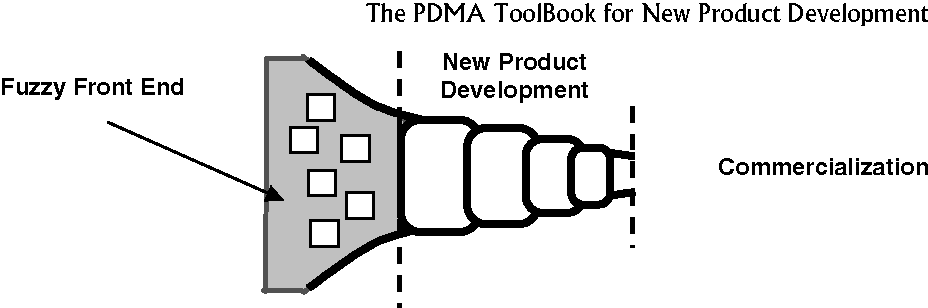
\includegraphics[width=1\textwidth]{figures/new_product_development.png}
    \caption{Representação Elastos}
    \end{center}
\end{figure}

O \emph{Fuzzy Front End} é a fase inicial do processo de desenvolvimento de novos produtos, correspondendo ao momento da identificação do problema ou à captação de oportunidades para o
projeto. Esta fase caracteriza-se por processos e decisões não estruturadas que tem como objetivo a identificação das necessidades dos potenciais clientes. A fase seguinte é o processo de  desenvolvimento do novo produto, sendo esta uma fase onde as ideias já estão mais estruturadas e os objetivos definidos. A terceira fase é a comercialização
do produto e corresponde à fase em que o produto é introduzido no mercado \cite{fuzzy_frontend}.

O modelo \emph{New Concept Development Model} é a representação das principais atividades do Fuzzy Front End. Este consiste em três componentes:

\begin{itemize}

\item Motor: Mecanismo que impulsiona as atividades de liderança e estratégia de negócio da organização;

\item Cinco Processos: São os processos que compõem o centro do modelo, que têm em conta a visão geral, a estratégia pretendida e a sua motivação;

\item Fatores de Influência: Variáveis não controláveis de origem interna ou externa ao projeto que afetam a sua inovação.

\end{itemize}

\begin{figure}[h]
    \begin{center}
    % Requires \usepackage{graphicx}
    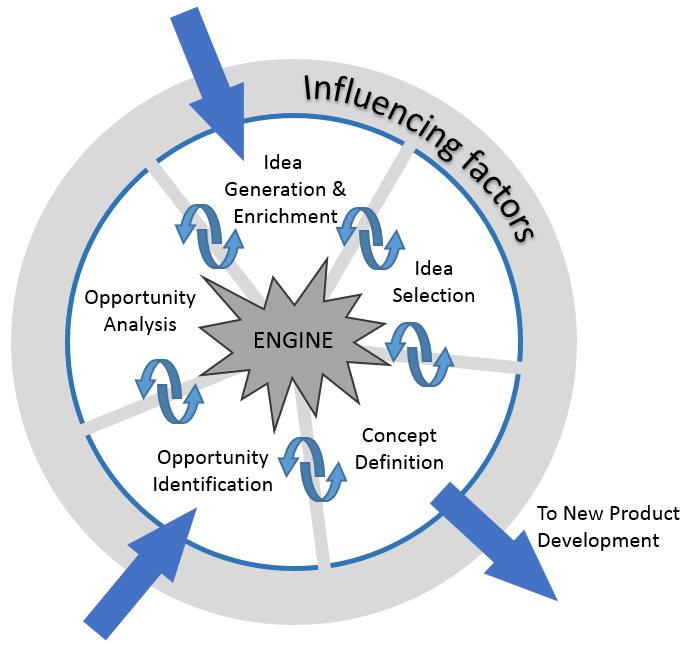
\includegraphics[width=0.5\textwidth]{figures/The-New-Concept-Development-NCD-model-Koen-et-al-2001.png}
    \caption{Representação New Concept Development Model}
    \end{center}
\end{figure}

O modelo apresenta duas vias de entrada e uma única saída, sendo este iniciado pela identificação de uma oportunidade ou pela geração de uma ideia. Essa irá posteriormente interagir com os restantes componentes do modelo.

\subsubsection{Analytic Hierarchy Process (AHP) \label{sym:AHP}}

Este método foi criado por Tomas L. Saaty em 1980, sendo um dos métodos mais conhecidos de apoio à decisão. O seu principio baseia-se em desconstruir a ideia em fragmentos cada vez mais pequenos de modo a tonar a sua análise mais fácil. Para atingir esse fim, o método divide-se em três fases: Divisão Hierárquica, Definição de Prioridades e Consistência \cite{ahp}.

A divisão hierárquica do AHP consiste na definição do objetivo, dos critérios de resolução do problema e, por último, nas alternativas que resolvem o problema. A lógica é que tendo este conceitos organizados hierarquicamente, conseguimos perceber a relação entre eles.

Depois da divisão hierárquica, é necessário definir prioridades entre os diferentes pares de critérios escolhidos. Esta priorização é subjetiva, sendo necessário calcular o índice de consistência de modo a validar a decisão. Para fazer a priorização de critérios é possível utilizar-se a tabela que apresenta a relação entre cada par de critérios utilizando a escala de Saaty. A escala de Saaty consiste numa escala numerada de 1 a 9, em que 1 corresponde a uma igualdade de importância entre critérios, 3 corresponde a uma fraca diferença de importância e 9 corresponde a uma diferença de importância absoluta. 


Por fim, é necessário garantir a consistência da decisão, uma vez que a priorização dos critérios é baseada em opinião e é subjetiva. Para isso são calculados os
índice de consistência e a razão de consistência. Desta forma é possível medir a consistência. Se o resultado do cálculo do rácio de consistência for menor que 0.1, consideram-se os critérios consistentes.

\subsubsection{Function Analysis System Technique (FAST) \label{sym:FAST}}

Este modelo permite apresentar de forma gráfica as relações entre as funcionalidades de um determinado projeto, produto, processo ou serviço, tendo por base as questões: "Como?" e "Porquê?"\cite{fast}.

Esta técnica ajuda, desta forma, a pensar no problema de forma mais objetiva e orientar os objetivos do seu desenvolvimento em função das relações entre as funcionalidades \cite{fast}.


\subsubsection{Modelo de Negócio \emph{Canvas}}

O modelo de negócio Canvas foi apresentado por Alex Osterwalder na sua tese de doutoramento \emph{The Business Model Ontology - A Proposition In A Design Science Approach, em 2004}. Este modelo permite, através de uma representação gráfica, mostrar como determinada empresa vende o seu produto  e como ganha dinheiro \cite{canvas}.

\subsection{Tecnologias}

\subsubsection{Arquitetura orientada a micro-serviços}
Uma arquitetura orientada a micros-serviços define uma configuração, na qual os componentes são aplicações independentes. Essas aplicações independentes comunicam utilizando estful Web Services ou troca de mensagens \cite{microservices}.
Seguem-se algumas características de sistemas orientados a micro-serviços:
\begin{description}
\item Micro-serviços em execução de forma independente;
\item Sistema é partido em micro-serviços, tendo por base \emph{bounded context} (c.f secção \ref{subsubsection:bounded:context} e/ou capacidades de negócio;
\item O conceito "produto" ganha relevo face ao conceito "projeto";
\item Aplicações devem utilizar canais de comunicação relativamente simples, como protocolo REST ou troca de mensagens.
\item Diferentes micro-serviços podem seguir arquiteturas e implementações diferentes, dependendo das suas especificidades e das decisões levadas a cabo pelas equipas de desenvolvimento;
\item Seguindo as boas práticas de desenvolvimento de micro-serviços, cada aplicação deve ter a sua própria unidade de persistência de dados, podendo inclusive a tecnologia adjacente à mesma ser diferente para cada micro-serviço;
\item \emph{Pipelines} de desenvolvimento independentes;
\item \emph{Deploys} independentes;
\end{description}

\subsubsection{\emph{Bounded Context}} \label{subsubsection:bounded:context}
\emph{Bounded Context} é um padrão crucial em DDD (\emph{Domain Driven Design}). É o foco da fase de desenho de grandes modelos. Para lidar com grandes modelos,DDD recorre a divisão em diferentes \emph{bounded contexts}. Estes tem como objetivo delimitar o domínio complexo em contextos baseados na intenção do negócio \cite{bounded_context}.

\subsubsection{REST}
\emph{Representational State Transfer} (\emph{REST}), é um estilo arquitetural que torna mais fácil a comunicação entre sistemas. Sistemas compativeis com \emph{REST}, são caracterizados por manterem um elevado desacoplamento entre o cliente e o servidor.
Neste estilo arquitetural, as aplicações cliente fazem pedidos para obter ou alterar recursos em aplicações servidor, estes pedidos são constituídos por \cite{rest}:
\begin{description}
    \item Verbo HTTP - Define o tipo de ação a realizar, pode ser \emph{GET}, \emph{POST}, \emph{PUT}, \emph{PATCH} ou \emph{DELETE}
    \item \emph{Header} - Permite ao cliente passar detalhes sobre o pedido
    \item Caminho - URL onde o pedido deve ser respondido
    \item \emph{Body} - Mensagem que contém a informação sobre o recurso a ser criado ou alterado
\end{description}

\subsubsection{\emph{API Gateway}} \label{api_gateway}
Uma \emph{API Gateway} é uma interface que se situa entre a aplicação cliente e os micro-serviços. Esta interface é utilizada para criar uma camada de abstração entre as aplicações e as APIs providenciadas pelos diferentes micro-serviços, permitindo, assim, um elevado desacoplamento entre as diferentes APIs do sistema.
Esta camada da arquitetura de um sistema permite ainda a implementação de mecanismos de monitorização e segurança das diferentes APIs.

\subsubsection{\emph{Troca de Mensagens Assíncrona}} \label{troca_mensagens_assincrona}
A troca de mensagens assíncrona consiste numa forma de troca de mensagens em que a aplicação que emite a mensagem não conhece o(s)seu(s) recetor(es), contribui para o incremento do desacoplamento entre as diferentes aplicações de um sistema.
Dois padrões associados a este mecanismo de troca de mensagens são \emph{Message Queueing} \emph{Publish/subscribe}.

\paragraph{\emph{Message Queueing}} \label{message_queueing} consiste num padrão em que as aplicações emissoras podem enviar para uma mesma fila, no entanto, existindo  apenas uma fila, qualquer mensagem poderá ser consumida apenas por um consumidor.

\begin{figure}[h]
    \begin{center}
    % Requires \usepackage{graphicx}
    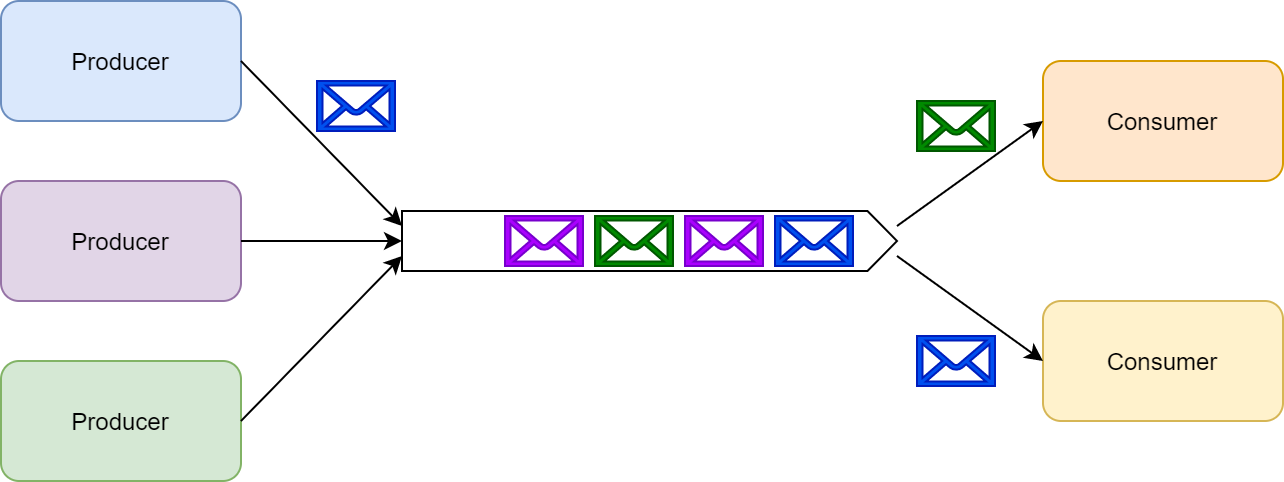
\includegraphics[width=1\textwidth]{figures/message_queueing.png}
    \caption{\emph{Message Queueing}}
    \end{center}
\end{figure}

\paragraph{\emph{Publish/Subscribe}} \label{publish_subscribe} tem um comportamento idêntico ao padrão \emph{Message Queueing}, adicionando a este uma camada que permite que a mesma mensagem seja enviada para mais do que uma fila.

\begin{figure}[h]
    \begin{center}
    % Requires \usepackage{graphicx}
    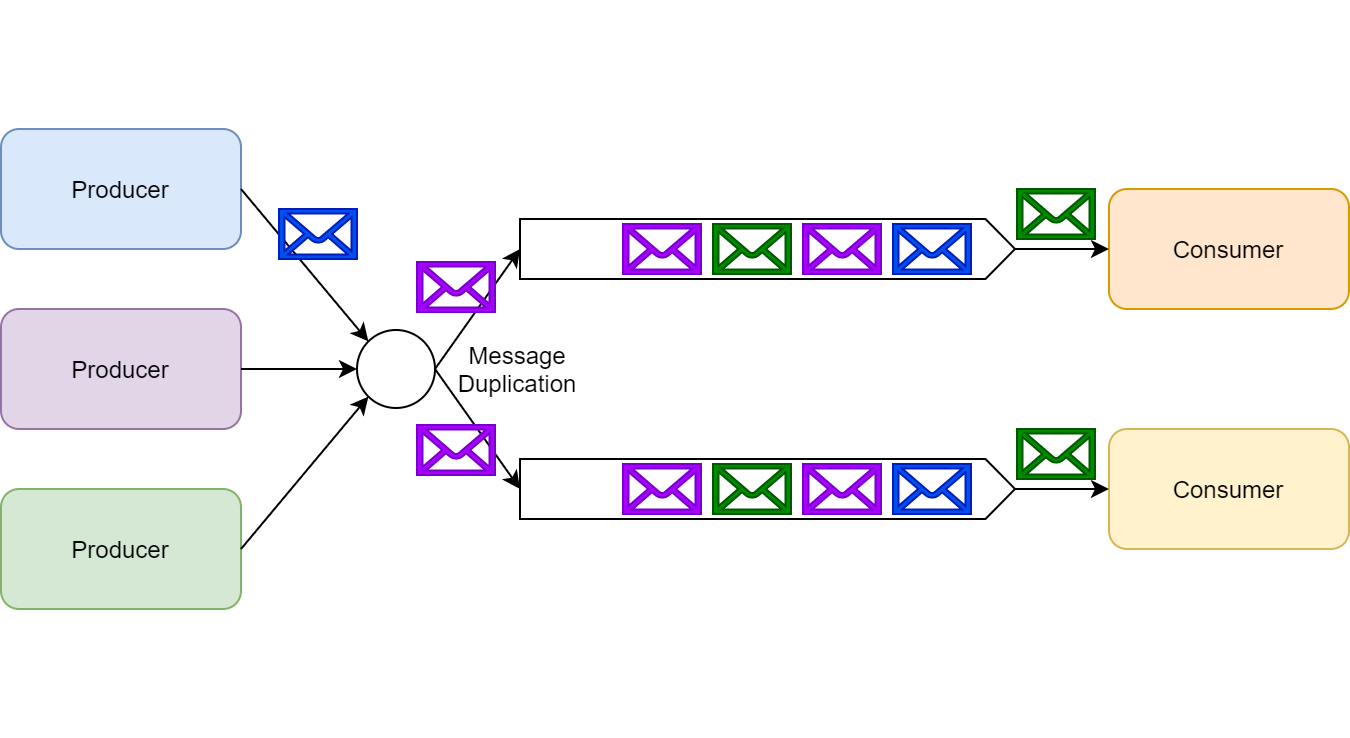
\includegraphics[width=1\textwidth]{figures/pub_sub.png}
    \caption{Publish/subscribe}
    \end{center}
\end{figure}

\paragraph{\emph{RabbitMQ}} é uma implementação de um \emph{Message Broker}, este suporta, de forma nativa, os dois padrão de de troca de mensagens assíncrona (c.f em \ref{message_queueing} e \ref{publish_subscribe}). Para a implementação da lógica no sentido do padrão \emph{Publish/subcribe}, \emph{RabbitMQ} introduz o conceito de \emph{Exchange}, este componente é responsável por reencaminhar a mesma mensagem para as diferentes filas que subscreveram aquele tipo de mensagem.

\paragraph{\emph{Apache Kafka}}, por outro lado, é uma plataforma distribuida de streaming. Ao contrário de \emph{RabbitMQ}, que é baseado em filas e \emph{exchanges}, a camada de armazenamento do \emph{Kafka} é implementada utilizando transações de logs particionadas.

\subsubsection{\emph{Command Query Responsability Segregation} (CQRS)} \label{cqrs}
Nas arquiteturas mais tradicionais, é utilizado o mesmo modelo de dados tanto para consultar como para atualizar a camada de persistência da aplicação. Esta abordagem é simples e funciona bem para operações CRUD básicas. Por outro lado, em aplicações mais complexas onde as cargas de leitura e de escrita são assimétricas, esta abordagem torna-se mais problemática e pode colocar em risco a escalabilidade do sistema. Neste contexto, o padrão CQRS incide em separar o modelo de leitura do modelo de escrita, existindo múltiplas abordagens para a sua implementação. \cite{cqrs}

\subsubsection{Teorema CAP} \label{cap_theorem}

O teorema é uma ferramenta utilizada para ajudar a tomar decisões durante o desenho de sistemas distribuídos. Eric Brewer inferiu que em qualquer sistema distribuído existe um equilíbrio entre consistência, disponibilidade e tolerância a falhas. Afirmação corroborada em 2002 por Seth Gilbert e Nancy Lynch. O teorema afirma que sistemas distribuídos apenas podem garantir três das seguintes propriedades \cite{cap_theorem}:

\begin{itemize}
    \item Consistência - Garantia que qualquer nó num sistema distribuído retorna a mesma, mais recente, escrita com sucesso. Consistência consiste em qualquer cliente ter a mesma vista de determinada informação num determinado momento;
    \item Disponibilidade - Todos os nós funcionais retornam resposta para os pedidos de leitura e escrita num tempo razoável de resposta;
    \item Tolerância a falhas - O sistema continua a funcionar e mantêm consistência mesmo em cenários de falha de rede.
\end{itemize}

\subsubsection{\emph{Event Sourcing} \label{event_sourcing}}
Event sourcing é um padrão que tem como objetivo garantir que as mudanças realizadas numa aplicação são armazenadas como uma sequência de eventos. Estes eventos persistidos, podem ser obtidos e utilizados para reconstruir estados da aplicação.
Neste sentido, este padrão é muitas vezes utilizado em conjunto com o padrão CQRS \cite{event_sourcing}.









